\section{Introduction}
\label{sec:intro}
% \textcolor{red}{TODO: (1) Survey Comparison table (with other surveys and perspectives.) (2) Modify the intro and structures (3) keep refining the figures}

\begin{figure*}[htbp]
  \centering
  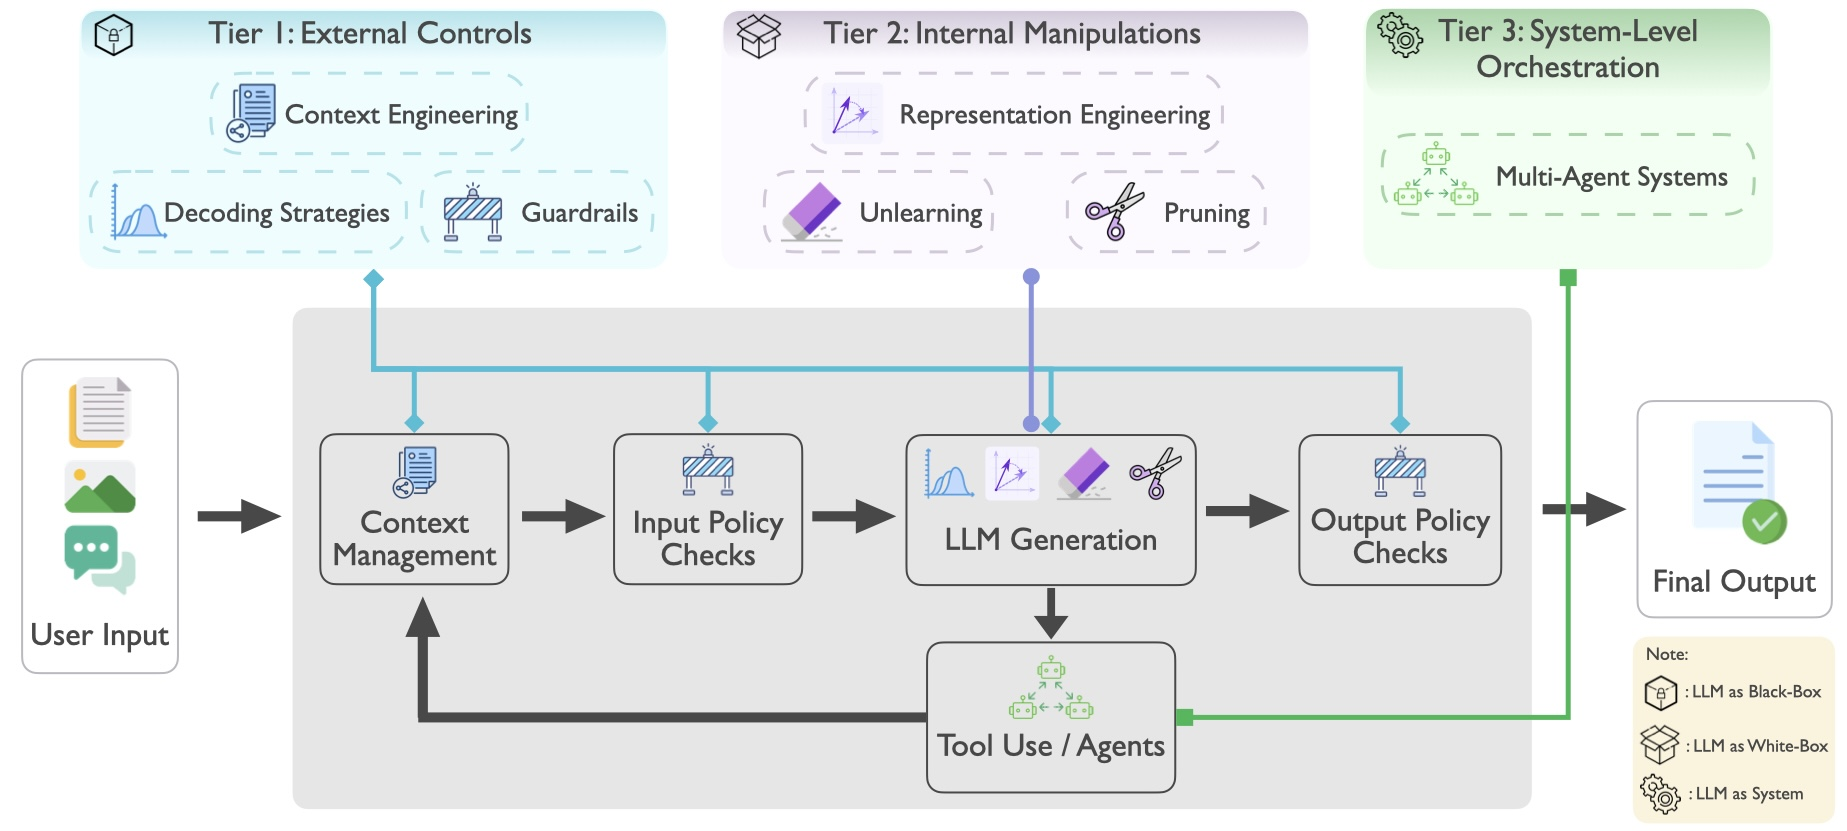
\includegraphics[width=1\linewidth]{figures/intro_v2.jpeg}
  \caption{Taxonomy (top) and attachment points in an inference-time pipeline (bottom). We organize seven inference-time methods into three tiers---\emph{External Controls} (Context Engineering, Guardrails, Decoding Strategies), \emph{Internal Manipulations} (Representation Engineering, Unlearning, Pruning), and \emph{System-Level Orchestration} (Multi-Agent Systems)---and map each to its point of intervention in the generation pipeline.}
  \label{fig:taxonomy_pipeline}
\end{figure*}

% Large Language Models (LLMs) and Multimodal Large Language Models (MLLMs) have rapidly moved from research prototypes to deployed systems in domains such as healthcare, law, and finance. Models are now accessed primarily through APIs, regulatory frameworks like the EU AI Act are imposing new behavioral requirements, and new vulnerabilities are discovered continuously after deployment. These pressures expose a fundamental limitation of training-time alignment alone. Once a model is released, updating its behavior is often slow, costly, or simply impossible for downstream users. In this survey, we study trustworthiness as the ability to maintain safe, fair, privacy-preserving, and reliable behavior at deployment time, and we argue that inference-time mechanisms are not merely a complement to training-time alignment but an increasingly necessary layer of control in their own right.

% \textcolor{red}{(1) Core Principles, shorten.
% (2) Applications, each trustworthy perspective has one paragraph (maybe delete some citations)
% (3) Move all of the discussion sections to the end (later sections can be divided by the methods)}

\textcolor{red}{Next step: 
\begin{enumerate}
    \item Figure 1, Figure 6 (misunderstanding), Figure 4 (font, size), Table 1 (larger font)
    \item for each figure, larger font (like figure 8)
\end{enumerate}
}

% \textcolor{red}{Yuyang: 
% \begin{enumerate}
%     \item Shorten/merge discussion part (2 page and a half -> 1 page and a half or 2 pages).
%     \item Remove some citations (Do so by updating the taxonomy), I would say shorten it to around 200 citations (now 240+). Just try your best first, I will help you later if this can't be done. 
%     \item Add name lists. The first three authors: Yuyang (Project leaders), Zheyuan (Project leaders), Han, .... (Other students are major contributors). Example below:
% \end{enumerate}
% }

% \textcolor{blue}{Han: (1) Redraw Figure 6 (Decoding pipeline)
% (2) Help modifying paper after adviser's review}

% \textcolor{cyan}{Logistic:
% \begin{enumerate}
%     \item Do we need taxonomy tree?
%     \item Let Meng, Yu review first before we invite other collaborators.
%     \item Recheck the format, CCS concepts keywords, additional key words and template (low priority)
%     \item Invitation List: Mohit, kaiwei, nanyun, Manling, Jieyu, Xiangliang, Heng (low priority)
%     \item Create a repo to hold all papers.
% \end{enumerate}
% }
\yuji{consider talking more about trustworthiness in high-stakes domains since the community starts to believe general reasoning has high reliability... Also connect the motivation to the recently more popular concept of ``harnessing''}
Large Language Models (LLMs) and Multimodal Large Language Models (MLLMs) have rapidly moved from research prototypes to deployed systems in domains such as healthcare, law, and finance. Models are now accessed primarily through APIs, regulatory frameworks like the EU AI Act are imposing new behavioral requirements, and new vulnerabilities are discovered continuously after deployment. Existing survey has largely emphasized train-time trustworthiness, where safety, fairness, privacy, or factuality objectives are encoded during parameter learning through data curation, supervised alignment, or preference optimization. These methods aim to shape the model’s default behavior globally and persistently by modifying what the model internalizes.

In this survey, we distinguish this perspective from inference-time trustworthiness, which concerns mechanisms that regulate model behavior at runtime after training has been completed. Rather than changing the model’s learned parameters alone, inference-time methods operate on the generation process through contextual control, decoding-time intervention, representation engineering, internal steering, or multi-agent verification. This distinction extends beyond considerations of efficiency or convenience. More fundamentally, train-time and inference-time methods differ in where control is exercised, how persistent the intervention is, and what level of guarantees it can provide. Train-time methods primarily shape a model’s behavioral prior, whereas inference-time methods determine how that prior is enacted, constrained, or corrected in a specific interaction context.

These two forms of trustworthiness are complementary. Train-time alignment is well suited for establishing broad and stable default behavior, but deployment introduces context-specific risks that cannot always be fully included during training, including changing policies, user-specific constraints, retrieval contamination, adversarial prompting, and jurisdiction-dependent requirements. Inference-time mechanisms provide a second control plane that is local, adaptive, and often more directly auditable at the level of individual interactions. They offer a complementary control layer that can steer, constrain, or monitor model behavior after deployment. Because they are often lightweight and modular, they are well suited to dynamic and context-specific trustworthiness requirements. Conversely, inference-time control alone cannot substitute for robust underlying models, because runtime interventions may be brittle, reactive, or incomplete without strong train-time foundations.\yuji{The two sentences sound like strong claims. Maybe consider supporting the two claims with abandant evidence (references)} A full account of trustworthy LLM deployment therefore requires treating trustworthiness as a multi-layer property spanning both training and inference.


% Training-time alignment methods such as instruction tuning and RLHF are central to shaping the general behavior of language models before deployment. However, once a model is released, updating that behavior is often slow, costly, or impossible, especially when users only have API access or limited control over model weights. This creates a practical gap between static alignment and real-world deployment, where requirements can change quickly. Organizations may need to revise safety policies, adapt behavior across users or jurisdictions, satisfy regulatory demands for transparent filtering or redaction, or respond to newly discovered vulnerabilities and distribution shifts. In these settings, retraining is often too rigid. Inference-time methods offer a complementary control layer that can steer, constrain, or monitor model behavior after deployment. Because they are often lightweight and modular, they are well suited to dynamic and context-specific trustworthiness requirements.

Many inference-time techniques were first developed to improve model performance, such as reducing latency, improving fluency, or grounding outputs through retrieval. More recently, they have also been adapted to support trustworthiness during deployment, including safety, privacy, fairness, and factuality. This shift calls for a more unified view of the field. In this survey, we organize inference-time trustworthiness methods by the mechanism and locus of control they introduce during generation. As shown in Figure~\ref{fig:taxonomy_pipeline}, we group them into three tiers: \textbf{External Controls}, \textbf{Internal Manipulations}, and \textbf{System-Level Orchestration}. This perspective highlights shared design patterns and clarifies trade-offs in granularity, invasiveness, and modularity. These tiers differ in where and how they intervene, ranging from black-box control around the model, to white-box intervention inside the model, to coordinated control across multiple agents.

\paragraph{Tier 1: External Controls.} These methods treat the model as a black box. They shape behavior by modifying the inputs, decoding process, or outputs, without changing internal weights or activations. These methods correspond to the \emph{context assembly}, \emph{input policy checks}, \emph{decoding}, and \emph{output policy checks} stages. This tier includes three categories:

\begin{itemize}
\item \textbf{Context Engineering} (Section~\ref{sec:context_engineering}): Strategic prompt design through rules, instructions, or few-shot exemplars to guide outputs without modifying model parameters.
\item \textbf{Guardrails} (Section~\ref{sec:guardrails}): External modules that inspect inputs or outputs against safety or policy constraints, blocking, redacting, or regenerating content when violations occur.
\item \textbf{Decoding Strategies} (Section~\ref{sec:decoding}): Manipulation of token-level distributions during generation to promote desired attributes or suppress undesired ones.
\end{itemize}

\paragraph{Tier 2: Internal Manipulations} require white-box access to the model. They intervene directly in the model's internal computation, such as by steering activations, removing learned behaviors, or pruning architectural components. In the pipeline, these methods operate within the \emph{LLM generation} stage. This tier includes three categories:

\begin{itemize}
\item \textbf{Representation Engineering} (Section~\ref{sec:representation_engineering}): Direct modification of internal activations by adding or subtracting steering vectors associated with specific concepts.
% \item \textbf{Editing} (Section~\ref{sec:editing}): Localized parameter updates to correct facts, update knowledge, or remove harmful associations efficiently.
\item \textbf{Unlearning} (Section~\ref{sec:unlearning}): Targeted removal of information, behaviors, or biases from a pre-trained model to fulfill data-forgetting requirements or disable harmful capabilities.
\item \textbf{Pruning} (Section~\ref{sec:pruning-core}): Post-training removal of weights, neurons, or attention heads, originally for efficiency but now increasingly explored for trust-related effects.
\end{itemize}

\paragraph{Tier 3: System-Level Orchestration} moves beyond single-model intervention. Rather than steering one model in isolation, this tier coordinates multiple LLM agents through structured interaction patterns such as debate, cross-verification, and role specialization. In the pipeline, the \emph{tool use / agents} loop spans context assembly, generation, and output checking, enabling iterative feedback and self-correction. This tier contains one category:

\begin{itemize}
\item \textbf{Multi-Agent Systems} (Section~\ref{sec:multi_agent_systems}): Coordinated agent interactions such as debate or cross-verification, where reliability is strengthened through collaboration.
\end{itemize}

These three tiers form a defense-in-depth view of inference-time trustworthiness. External controls provide lightweight and modular policy enforcement. Internal manipulations enable more direct and fine-grained behavioral intervention. System-level orchestration introduces an additional layer of reliability through collaborative reasoning and feedback. Across this taxonomy, we focus on four dimensions of trustworthiness: \textbf{Safety}, which concerns preventing harmful, biased, or malicious outputs and defending against misuse such as jailbreaks; \textbf{Privacy}, which concerns limiting training-data leakage and protecting user inputs during inference; \textbf{Fairness}, which concerns reducing systematic disadvantages toward individuals or groups; and \textbf{Factuality}, which concerns grounding model outputs in verifiable knowledge and reducing hallucinations. By synthesizing these developments, this survey aims to provide a unified framework for understanding inference-time trustworthiness methods, their trade-offs, and their opportunities for combination under real-world deployment constraints.

\subsection{Related Surveys}
Our work sits at the intersection of three strands: inference efficiency, post-training capability enhancement, and broad-spectrum trustworthiness.

\paragraph{Efficiency-Focused Surveys.}
Comprehensive surveys review inference-time optimizations such as quantization, distillation, and speculative decoding~\citep{survey:inference_efficiency1}. Others target specialized settings like Mixture-of-Experts~\citep{survey:inference_moe} or memory-footprint reduction for large deployments~\citep{survey:inference_efficiency2}. These studies are foundational for understanding mechanics and cost, but their primary objective is computational performance rather than the explicit control of trustworthy behavior.

\paragraph{Surveys on Post-Training Capability Enhancement.}
A second line examines methods applied after pre-training to improve complex-task performance, including prompting-based techniques and reinforcement learning advances~\citep{survey:post-training1, survey:post-training2}. The focus is to make models more capable reasoners or tool users. Alignment is peripheral; fine-grained enforcement of safety, privacy, or fairness at deployment is not the central goal.

\paragraph{Trustworthy-Focused Surveys.}
Holistic surveys chart the landscape of trustworthy LLMs from data integrity to evaluation~\citep{survey:trustworthy1, survey:trustworthy2}. Other work dives deep into specific facets---mitigating social bias in text-to-image generation~\citep{survey:trustworthy_text2img}, safety for autonomous LLM agents~\citep{survey:trustworthy_agents}, or machine unlearning~\citep{survey:unlearning1, survey:unlearning2}. While invaluable, these efforts either organize by harm type or by a single solution family. To our knowledge, none provides a systematic, unified taxonomy that treats \emph{inference-time methods as a control plane} for trustworthiness across safety, privacy, fairness, and factuality.

\subsection{Contributions and Organization}
This survey analyzes inference-time methods for enhancing the trustworthiness of LLMs. Our primary contribution is a unified, pipeline-grounded taxonomy that organizes post-hoc control techniques into seven categories across three tiers---External Controls (Context Engineering, Guardrails, Decoding Strategies), Internal Manipulations (Representation Engineering, Unlearning, Pruning), and System-Level Orchestration (Multi-Agent Systems)---and evaluates them against four deployment-critical dimensions: Safety, Privacy, Fairness, and Factuality. Our key contributions are as follows:

\begin{itemize}
    \item \textbf{A Pipeline-Grounded, Three-Tier Taxonomy of Inference-Time Methods.} We organize seven categories of inference-time control into a coherent three-tier hierarchy---External Controls, Internal Manipulations, and System-Level Orchestration---grounded in the inference-time pipeline (Figure~\ref{fig:taxonomy_pipeline}). This structure clarifies each method's point of intervention, access requirements, and composability within a defense-in-depth design.
    \item \textbf{Systematic Cross-Dimensional Analysis.} We analyze how each category addresses Safety, Privacy, Fairness, and Factuality, clarifying capabilities, limitations, and trade-offs under deployment constraints.
    \item \textbf{Future Directions and Open Challenges.} We synthesize open problems on scalability, evaluation, and composition, and outline a research agenda for real-world systems.
\end{itemize}

The remainder of the survey is organized as follows. \textbf{Section~\ref{sec:external_controls}} presents the three External Controls---Context Engineering, Guardrails, and Decoding Strategies---that operate on inputs, outputs, or the token-selection process without accessing model internals. \textbf{Section~\ref{sec:internal_manipulations}} covers four Internal Manipulations---Representation Engineering, Unlearning, and Pruning---that intervene on the model's activations or parameters. \textbf{Section~\ref{sec:system_level}} discusses System-Level Orchestration through Multi-Agent Systems. \textbf{Section~\ref{sec:evaluation}} provides a critical analysis of evaluation benchmarks and trade-offs. \textbf{Section~\ref{sec:challenges}} consolidates open challenges and future directions. \textbf{Section~\ref{sec:conclusion}} concludes the survey.
